% Copyright 2004 by Till Tantau <tantau@users.sourceforge.net>.
%
% In principle, this file can be redistributed and/or modified under
% the terms of the GNU Public License, version 2.
%
% However, this file is supposed to be a template to be modified
% for your own needs. For this reason, if you use this file as a
% template and not specifically distribute it as part of a another
% package/program, I grant the extra permission to freely copy and
% modify this file as you see fit and even to delete this copyright
% notice. 

\documentclass{beamer}

\usepackage[numbers]{natbib}
\usepackage{todonotes}
\usepackage{booktabs}
\usepackage{afterpage}
\usepackage{amsfonts}
\usepackage{amsmath}
\usepackage{amssymb}
\usepackage{amsthm}
\usepackage[english]{babel}
\usepackage{graphicx}
\usepackage[utf8]{inputenc}
\usepackage{latexsym}
\usepackage{url}
\usepackage{tikz}
\usepackage{pdfpages}
\usetikzlibrary{arrows}
\usepackage{float}
\usepackage[algoruled,boxed,lined]{algorithm2e}


% There are many different themes available for Beamer. A comprehensive
% list with examples is given here:
% http://deic.uab.es/~iblanes/beamer_gallery/index_by_theme.html
% You can uncomment the themes below if you would like to use a different
% one:
%\usetheme{AnnArbor}
%\usetheme{Antibes}
%\usetheme{Bergen}
%\usetheme{Berkeley}
%\usetheme{Berlin}
%\usetheme{Boadilla}
%\usetheme{boxes}
%\usetheme{CambridgeUS}
%\usetheme{Copenhagen}
%\usetheme{Darmstadt}
%\usetheme{default}
%\usetheme{Frankfurt}
%\usetheme{Goettingen}
%\usetheme{Hannover}
%\usetheme{Ilmenau}
%\usetheme{JuanLesPins}
%\usetheme{Luebeck}
\usetheme{Madrid}
%\usetheme{Malmoe}
%\usetheme{Marburg}
%\usetheme{Montpellier}
%\usetheme{PaloAlto}
%\usetheme{Pittsburgh}
%\usetheme{Rochester}
%\usetheme{Singapore}
%\usetheme{Szeged}
%\usetheme{Warsaw}

\title{Deep learning methods for lacune detection in MRI}

\author{Melinda Mortimer}
% - Give the names in the same order as the appear in the paper.
% - Use the \inst{?} command only if the authors have different
%   affiliation.

\institute[UNSW] % (optional, but mostly needed)
{
  Supervisors: Dr Pierre Lafaye de Micheaux and A/Prof. Wei Wen
}
% - Use the \inst command only if there are several affiliations.
% - Keep it simple, no one is interested in your street address.

\date{24 October, 2018}
% - Either use conference name or its abbreviation.
% - Not really informative to the audience, more for people (including
%   yourself) who are reading the slides online

% This is only inserted into the PDF information catalog. Can be left
% out. 

% If you have a file called "university-logo-filename.xxx", where xxx
% is a graphic format that can be processed by latex or pdflatex,
% resp., then you can add a logo as follows:

% \pgfdeclareimage[height=0.5cm]{university-logo}{university-logo-filename}
% \logo{\pgfuseimage{university-logo}}

% Delete this, if you do not want the table of contents to pop up at
% the beginning of each subsection:
\AtBeginSection[]
{
  \begin{frame}<beamer>{Outline}
    \tableofcontents[currentsection,currentsubsection]
  \end{frame}
}

\setbeamertemplate{footline}
{
  \leavevmode%
  \hbox{%
  \begin{beamercolorbox}[wd=.4\paperwidth,ht=2.25ex,dp=1ex,center]{author in head/foot}%
    \usebeamerfont{author in head/foot}\insertshortauthor
  \end{beamercolorbox}%
  \begin{beamercolorbox}[wd=.6\paperwidth,ht=2.25ex,dp=1ex,center]{title in head/foot}%
    \usebeamerfont{title in head/foot}\insertshorttitle\hspace*{3em}
    \insertframenumber{} / \inserttotalframenumber\hspace*{1ex}
  \end{beamercolorbox}}%
  \vskip0pt%
}


% Let's get started
\begin{document}

\begin{frame}
	\titlepage
\end{frame}


\begin{frame}{Overview}
	\tableofcontents
\end{frame}

% Define lacunes: associated with an increased risk of stroke.
% Only small 3-15 mm.
% MRI have many image types designed to detect different things. We'll be dealing with T1 and flair.
% lacunes appear dark in t1 and are also dark in flair with a bright rim.
\section{Introduction}
\begin{frame}{Introduction}
    \begin{itemize}
    \item Lacunes are small brain cavities associated with the incidence of stroke.
    \item Appear round in \textsc{mri} with a diameter of 3--15 mm.
	\item Lacunes appear dark in T1-weighted images, with a bright rim in \textsc{flair}.
    \end{itemize}
    	\begin{figure}
	\centering
	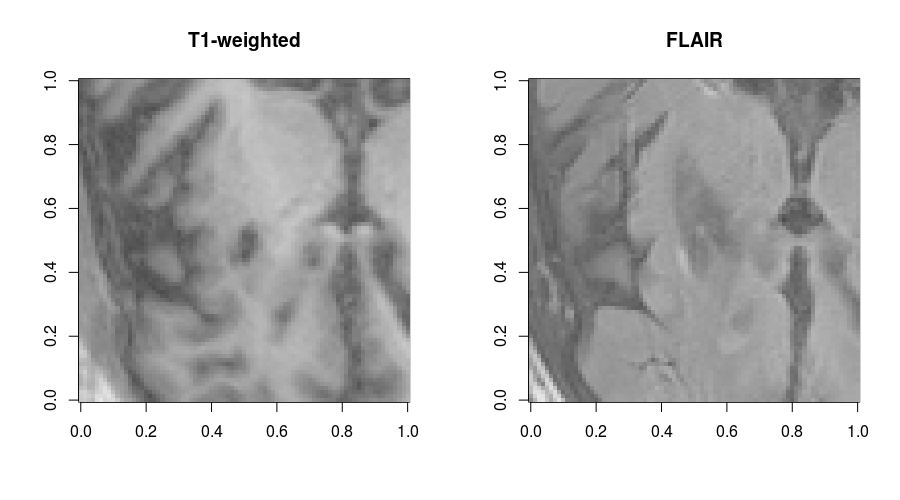
\includegraphics[width=0.8\linewidth]{../Thesis_Docs/Images/2_lacune_t1_flair.png}
	\end{figure}
\end{frame}




% Current lacune detection is quite rudimentary. Clinicians search for the lacunes by eye, searching through the volume one image at a time.
% time consuming: scan is detailed. Each scan approx 1 hour.
% lacune identification inconsistent. Lacunes appear similar to other lesions in the brain. Subjective across clinicians. 
% Therefore make an automated model to improve the speed, consistency and reliability of lacune detection.
\begin{frame}{Current lacune detection methods}
\begin{itemize}
\setlength\itemsep{1em}
\item Lacune detection is conducted by eye.
\item Process is time consuming.
\item Identification is inconsistent.
\pause
\item \textbf{Aim:} Implement an automated approach to improve the speed, consistency, and reliability of lacune detection.
\end{itemize}
\end{frame}




% NNets background. Go through basic neuron structure (bunch of inputs, single output). 
% Neuron takes in a number of variables denoted by x, conducts a weighted sum of these variables and adds a constant b. The resulting linear combination is input in an activation function, which commonly introduces some nonlinearity, and finally outputs a single value. Ideally, the neuron will have its weights and biases chosen such that it captures some feature of the data.
\section{Background on neural networks}
\begin{frame}{Structure of a basic neuron}
The basic neural network unit is the \textit{neuron}.
% Basic Neuron diagram
\begin{figure}[hb]
\centering
\tikzset{every picture/.style={line width=0.75pt}} %set default line width to 0.75pt        
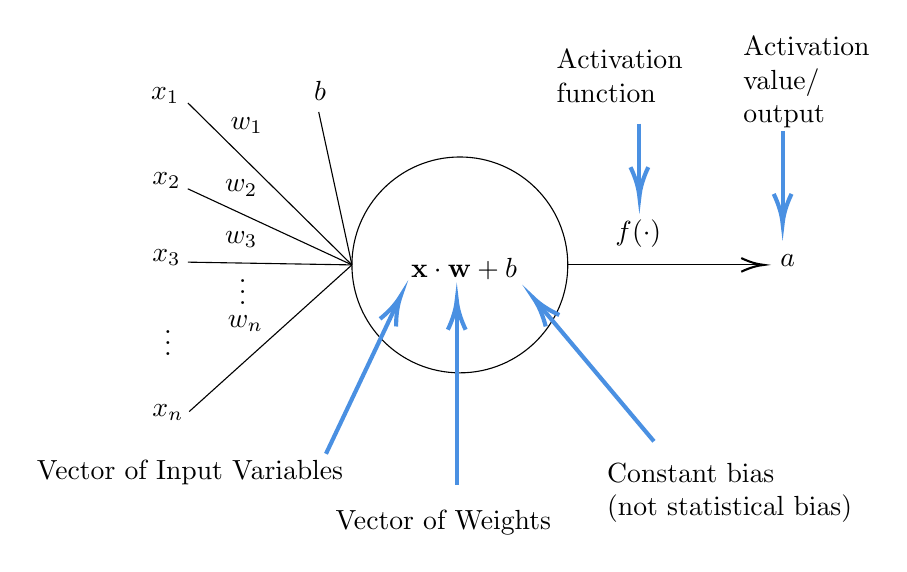
\begin{tikzpicture}[x=0.75pt,y=0.75pt,yscale=-1,xscale=1]
%uncomment if require: \path (0,364); %set diagram left start at 0, and has height of 364

%Shape: Circle [id:dp7806506925261892] 
\draw   (270,154) .. controls (270,125.28) and (293.28,102) .. (322,102) .. controls (350.72,102) and (374,125.28) .. (374,154) .. controls (374,182.72) and (350.72,206) .. (322,206) .. controls (293.28,206) and (270,182.72) .. (270,154) -- cycle ;
%Straight Lines [id:da48045113953293783] 
\draw    (191,76) -- (270,154) ;


%Straight Lines [id:da20730706323067383] 
\draw    (190.92,117.33) -- (270,154) ;


%Straight Lines [id:da19390293965519045] 
\draw    (191.59,224.67) -- (270,154) ;


%Straight Lines [id:da5499170807272789] 
\draw    (374,154) -- (466.51,154) ;
\draw [shift={(468.51,154)}, rotate = 180] [color={rgb, 255:red, 0; green, 0; blue, 0 }  ][line width=0.75]    (10.93,-3.29) .. controls (6.95,-1.4) and (3.31,-0.3) .. (0,0) .. controls (3.31,0.3) and (6.95,1.4) .. (10.93,3.29)   ;

%Straight Lines [id:da7426731370805287] 
\draw    (270,154) -- (190.92,152.67) ;


%Straight Lines [id:da35133187079282135] 
\draw    (254,80.33) -- (270,154) ;


%Straight Lines [id:da7452273715557709] 
\draw [color={rgb, 255:red, 74; green, 144; blue, 226 }  ,draw opacity=1 ][line width=1.5]    (257.5,245) -- (292.22,171.71) ;
\draw [shift={(293.5,169)}, rotate = 475.35] [color={rgb, 255:red, 74; green, 144; blue, 226 }  ,draw opacity=1 ][line width=1.5]    (14.21,-4.28) .. controls (9.04,-1.82) and (4.3,-0.39) .. (0,0) .. controls (4.3,0.39) and (9.04,1.82) .. (14.21,4.28)   ;

%Straight Lines [id:da6267543092908385] 
\draw [color={rgb, 255:red, 74; green, 144; blue, 226 }  ,draw opacity=1 ][line width=1.5]    (320.5,260.02) -- (320.5,174) ;
\draw [shift={(320.5,171)}, rotate = 450] [color={rgb, 255:red, 74; green, 144; blue, 226 }  ,draw opacity=1 ][line width=1.5]    (14.21,-4.28) .. controls (9.04,-1.82) and (4.3,-0.39) .. (0,0) .. controls (4.3,0.39) and (9.04,1.82) .. (14.21,4.28)   ;

%Straight Lines [id:da27997502059011203] 
\draw [color={rgb, 255:red, 74; green, 144; blue, 226 }  ,draw opacity=1 ][line width=1.5]    (415.5,239) -- (359.43,172.3) ;
\draw [shift={(357.5,170)}, rotate = 409.95] [color={rgb, 255:red, 74; green, 144; blue, 226 }  ,draw opacity=1 ][line width=1.5]    (14.21,-4.28) .. controls (9.04,-1.82) and (4.3,-0.39) .. (0,0) .. controls (4.3,0.39) and (9.04,1.82) .. (14.21,4.28)   ;

%Straight Lines [id:da3489893362960632] 
\draw [color={rgb, 255:red, 74; green, 144; blue, 226 }  ,draw opacity=1 ][line width=1.5]    (408.5,85.99) -- (408.5,118.13) ;
\draw [shift={(408.5,121.13)}, rotate = 270] [color={rgb, 255:red, 74; green, 144; blue, 226 }  ,draw opacity=1 ][line width=1.5]    (14.21,-4.28) .. controls (9.04,-1.82) and (4.3,-0.39) .. (0,0) .. controls (4.3,0.39) and (9.04,1.82) .. (14.21,4.28)   ;

%Straight Lines [id:da7842417457885081] 
\draw [color={rgb, 255:red, 74; green, 144; blue, 226 }  ,draw opacity=1 ][line width=1.5]    (477.5,89.66) -- (477.5,131.01) ;
\draw [shift={(477.5,134.01)}, rotate = 270] [color={rgb, 255:red, 74; green, 144; blue, 226 }  ,draw opacity=1 ][line width=1.5]    (14.21,-4.28) .. controls (9.04,-1.82) and (4.3,-0.39) .. (0,0) .. controls (4.3,0.39) and (9.04,1.82) .. (14.21,4.28)   ;


% Text Node
\draw (324,156) node   {${\displaystyle \mathbf{x} \cdot \mathbf{w} +b}$};
% Text Node
\draw (180,72.33) node   {$x_{1}$};
% Text Node
\draw (180.67,113.33) node   {$x_{2}$};
% Text Node
\draw (181.33,187.67) node   {$\vdots $};
% Text Node
\draw (181.33,225.33) node   {$x_{n}$};
% Text Node
\draw (180.67,150.33) node   {$x_{3}$};
% Text Node
\draw (219.33,87) node   {$w_{1}$};
% Text Node
\draw (216.67,117) node   {$w_{2}$};
% Text Node
\draw (216.67,141.67) node   {$w_{3}$};
% Text Node
\draw (218.67,182.33) node   {$w_{n}$};
% Text Node
\draw (217.33,163) node   {$\vdots $};
% Text Node
\draw (254.67,70.33) node   {$b$};
% Text Node
\draw (408,139) node   {$f ( \cdot )$};
% Text Node
\draw (480,151.67) node   {$a$};
% Text Node
\draw (192,254) node  [align=left] {Vector of Input Variables};
% Text Node
\draw (314,278) node  [align=left] {Vector of Weights};
% Text Node
\draw (452,264) node  [align=left] {Constant bias \\(not statistical bias)};
% Text Node
\draw (399,63) node  [align=left] {Activation\\function};
% Text Node
\draw (489,66) node  [align=left] {Activation\\value/\\output};
\end{tikzpicture}
\end{figure}
\end{frame}




% Simple example of a neuron. AND gate
\begin{frame}{Example of a basic neuron}
The logical \textsc{and} gate can be represented as a neuron.
\begin{examples}
Let $x_1,x_2\in\{0,1\}$. The output of the neuron is 1 if and only if $x_1 = x_2 = 1$.
% AND neuron figure
\begin{figure}

\tikzset{every picture/.style={line width=0.75pt}} %set default line width to 0.75pt        

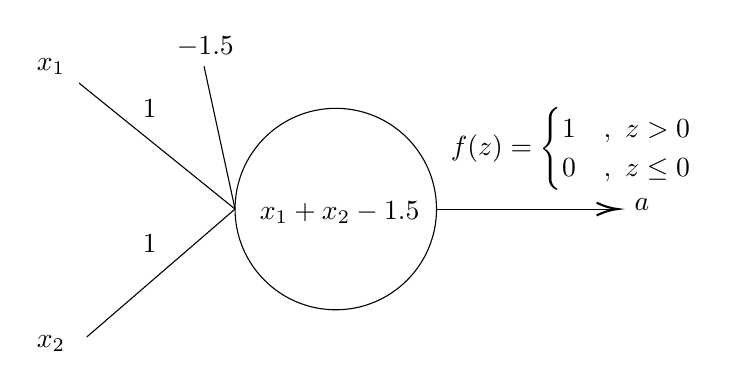
\begin{tikzpicture}[x=0.7pt,y=0.7pt,yscale=-1,xscale=1]
%uncomment if require: \path (0,364); %set diagram left start at 0, and has height of 364

%Shape: Circle [id:dp7806506925261892] 
\draw   (270,154) .. controls (270,125.28) and (293.28,102) .. (322,102) .. controls (350.72,102) and (374,125.28) .. (374,154) .. controls (374,182.72) and (350.72,206) .. (322,206) .. controls (293.28,206) and (270,182.72) .. (270,154) -- cycle ;
%Straight Lines [id:da48045113953293783] 
\draw    (189.5,89) -- (270,154) ;


%Straight Lines [id:da20730706323067383] 
\draw    (193.5,220) -- (270,154) ;


%Straight Lines [id:da5499170807272789] 
\draw    (374,154) -- (465.59,154) ;
\draw [shift={(467.59,154)}, rotate = 540] [color={rgb, 255:red, 0; green, 0; blue, 0 }  ][line width=0.75]    (10.93,-3.29) .. controls (6.95,-1.4) and (3.31,-0.3) .. (0,0) .. controls (3.31,0.3) and (6.95,1.4) .. (10.93,3.29)   ;

%Straight Lines [id:da35133187079282135] 
\draw    (254,80.33) -- (270,154) ;



% Text Node
\draw (324,156) node   {$x_{1} +x_{2} -1.5$};
% Text Node
\draw (175,80.33) node   {$x_{1}$};
% Text Node
\draw (175,223.33) node   {$x_{2}$};
% Text Node
\draw (226,102) node   {$1$};
% Text Node
\draw (226,172) node   {$1$};
% Text Node
\draw (254.67,70.33) node   {$-1.5$};
% Text Node
\draw (444,123) node   {$f ( z) =\begin{cases}
1 & ,\ z >0\\
0 & ,\ z\leq 0
\end{cases}$};
% Text Node
\draw (480,151.67) node   {$a$};


\end{tikzpicture}





\end{figure}
\end{examples}
\end{frame}



% Single neuron is quite simplistic. If we want to model something with more detail, we're going to need a structure that is more complex. As a result, we combine multiple neurons together into this layered structure. We have a set of input variables and we want to use them to predict some response y. The blue dots and the final green dot each symbolise a neuron. The inputs on the far left are fed into each neuron of the first layer. Each neuron of the first layer outputs a single activation value. These are then passed as inputs into the second layer, where a similar process occurs. The final output neuron takes in the activations of the previous layer and outputs a single value.
% As before, the neurons have weights and biases and these need to be chosen. The way we do that is by minimising some cost function. However, even this neural network, which is only small, has 41 weights. Minimising a large number of weights analytically is slow. 
\begin{frame}{Structure of a basic neural network}
% Whole network diagram
\begin{figure}[t]
\centering
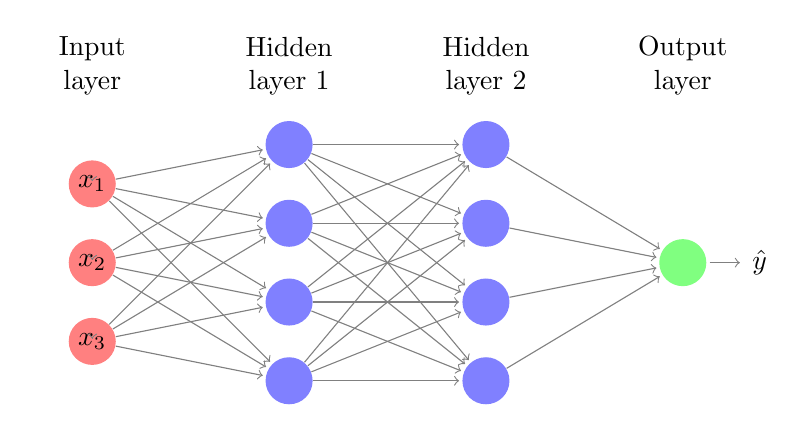
\begin{tikzpicture}[shorten >=1pt,->,draw=black!50, node distance=\layersep]
    \tikzstyle{every pin edge}=[<-,shorten <=1pt]
    \tikzstyle{neuron}=[circle,fill=black!25,minimum size=17pt,inner sep=0pt]
    \tikzstyle{input neuron}=[neuron, fill=red!50];
    \tikzstyle{output neuron}=[neuron, fill=green!50];
    \tikzstyle{hidden neuron}=[neuron, fill=blue!50];
    \tikzstyle{annot} = [text width=4em, text centered]
	\def\layersep{2.5cm}
	
    % Draw the input layer nodes
    \foreach \name / \y in {1,...,3}
    % This is the same as writing \foreach \name / \y in {1/1,2/2,3/3,4/4}
        \node[input neuron, pin=center:$x_\y$] (I-\name) at (0,-\y) {};

    % Draw the hidden layer1 nodes
    \foreach \name / \y in {1,...,4}
        \path[yshift=0.5cm]
            node[hidden neuron] (Ha-\name) at (\layersep,-\y cm) {};
            
    % Draw the hidden layer2 nodes
    \foreach \name / \y in {1,...,4}
        \path[yshift=0.5cm]
            node[hidden neuron] (Hb-\name) at (2*\layersep,-\y cm) {};

    % Draw the output layer node
    \node[output neuron,pin={[pin edge={->}]right:$\hat{y}$}] (O) at (3*\layersep, -2) {};

    % Connect every node in the input layer with every node in the
    % hidden layer.
    \foreach \source in {1,...,3}
        \foreach \dest in {1,...,4}
            \path (I-\source) edge (Ha-\dest);
            
    % Connect every node in the hidden layer 1 with every node in
    % hidden layer 2.
    \foreach \source in {1,...,4}
        \foreach \dest in {1,...,4}
            \path (Ha-\source) edge (Hb-\dest);

    % Connect every node in the hidden layer with the output layer
    \foreach \source in {1,...,4}
        \path (Hb-\source) edge (O);

    % Annotate the layers
    \node[annot,above of=Ha-1, node distance=1cm] (hla) {Hidden layer 1};
    \node[annot,above of=Hb-1, node distance=1cm] (hlb) {Hidden layer 2};
    \node[annot,left of=hla] {Input layer};
    \node[annot,right of=hlb] {Output layer};

\end{tikzpicture}
\end{figure}
\pause
\begin{itemize}
\item Network weights and biases are chosen such that they minimise some \textit{cost function}. E.g. Mean Squared Error.
\item Having a network with a large number of weights makes minimisation slow.
\end{itemize}
\end{frame}



% We instead aim to approximate the minimum via the gradient descent algorithm. This algorithm is iterative. It initialises the weights, and at each iteration, moves the weights in the direction that decreases the cost function, by some predetermined amount. 
% Introduces two problems. The first is that since relies on gradients, the minimum being converged to is not necessarily global. Could just be local.
% Secondly, this method is prone to overfitting the data. There are methods to mitigate this, but these are covered in greater detail in my thesis.
\begin{frame}{Choosing the network weights}
\begin{itemize}
\item It is faster to instead estimate the weights using the \textit{Gradient Descent algorithm}.
\item Two issues: no guarantee that the minimum is global, and overfitting.
\end{itemize}
\begin{figure}
\centering

\tikzset{every picture/.style={line width=0.75pt}} %set default line width to 0.75pt        

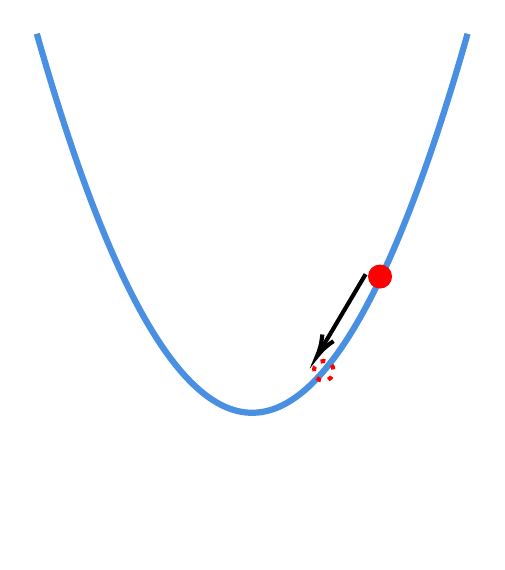
\begin{tikzpicture}[x=0.55pt,y=0.55pt,yscale=-1,xscale=1]
%uncomment if require: \path (0,291); %set diagram left start at 0, and has height of 291

%Shape: Parabola [id:dp09742535750627612] 
\draw  [color={rgb, 255:red, 74; green, 144; blue, 226 }  ,draw opacity=1 ][line width=2.25]  (90,18) .. controls (184.33,350) and (278.67,350) .. (373,18) ;
%Straight Lines [id:da11196791721275057] 
\draw [color={rgb, 255:red, 0; green, 0; blue, 0 }  ,draw opacity=1 ][line width=1.5]    (306,176) -- (275.53,227.42) ;
\draw [shift={(274,230)}, rotate = 300.65] [color={rgb, 255:red, 0; green, 0; blue, 0 }  ,draw opacity=1 ][line width=1.5]    (14.21,-4.28) .. controls (9.04,-1.82) and (4.3,-0.39) .. (0,0) .. controls (4.3,0.39) and (9.04,1.82) .. (14.21,4.28)   ;

%Shape: Circle [id:dp1570017763837479] 
\draw  [color={rgb, 255:red, 255; green, 0; blue, 0 }  ,draw opacity=1 ][dash pattern={on 1.69pt off 2.76pt}][line width=1.5]  (272,239.5) .. controls (272,235.91) and (274.91,233) .. (278.5,233) .. controls (282.09,233) and (285,235.91) .. (285,239.5) .. controls (285,243.09) and (282.09,246) .. (278.5,246) .. controls (274.91,246) and (272,243.09) .. (272,239.5) -- cycle ;
%Shape: Circle [id:dp7325121590212951] 
\draw  [color={rgb, 255:red, 255; green, 0; blue, 0 }  ,draw opacity=1 ][fill={rgb, 255:red, 255; green, 0; blue, 0 }  ,fill opacity=1 ][line width=1.5]  (309,177.5) .. controls (309,173.91) and (311.91,171) .. (315.5,171) .. controls (319.09,171) and (322,173.91) .. (322,177.5) .. controls (322,181.09) and (319.09,184) .. (315.5,184) .. controls (311.91,184) and (309,181.09) .. (309,177.5) -- cycle ;
%Shape: Rectangle [id:dp29688417965832214] 
\clip(84,14) rectangle (379,274) ;
\end{tikzpicture}
\end{figure}
\end{frame}




% Regular neuron networks work well for a collection of variables, but our lacune detection problem is not concerned with the values of particular pixels on their own, but rather patterns that are occurring with a collection of pixels in a 2D space. Conv nets allow for that and are frequently used for image classification.
% IN this example, on the left we have the input image of a bird, and we are trying to classify the image as one of these categories. The cnn adds what are called convolutional layers, which try to identify certain visual features. For example feathers or an eye, and scans the image in a small search window from top left to bottom right, outputing a high value at each point that contains the relevant feature. 
% As the conv layer creates essentially another image for each feature being identified, the number of variables increases very quickly. Pooling layers are placed after convolution to reduce some of the dimensionality. 
\begin{frame}{Structure of convolutional neural networks (\textsc{cnn}s)}
\begin{itemize}
\item \textsc{cnn}s can be used for two-dimensional data.
\item Convolutional layers locate a set of features from the previous layer.
\end{itemize}
\begin{figure}
\centering
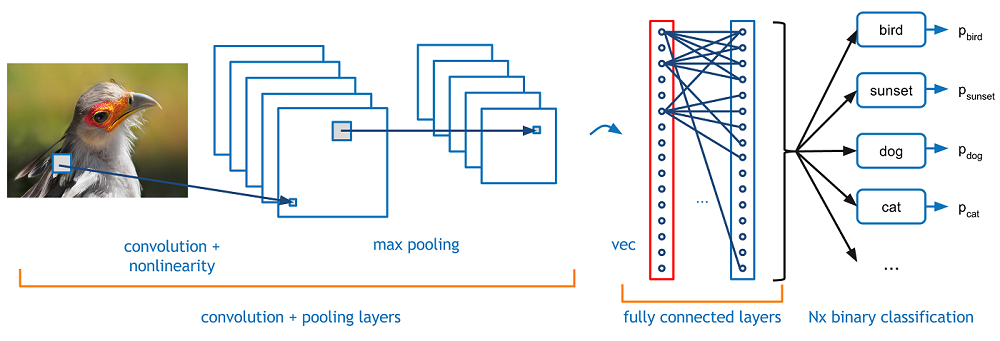
\includegraphics[width=\linewidth]{../Thesis_Docs/Images/4_cnn_structure.png}

\small{Diagram sourced from \citep{ADeshpande2016}.}
\end{figure}
\end{frame}



\section{Model development}

% Link back to results. Model was based on existing model by Ghafoorian et al. Model consisted of two stages: candidate detection, followed by false-positive reduction. The candidate detection model feeds 51x51 subimages through four convolutional layers, followed by 3 fully connected layers. The candidate lacunes output by this first model is fed into a second false-positive reduction model. The false-positive reduction model is comprised of three parallel three-dimensional convolutional neural networks. The outputs of these are concatenated with 7 location-based variables in three fully connected layers.
\begin{frame}{Lacune detection model by Ghafoorian et al.}
\begin{itemize}
\item Ghafoorian et al. \cite{GhafoorianM.2017Dml3} lacune candidate detection model. 51$\times$51 inputs.
\begin{figure}
\centering
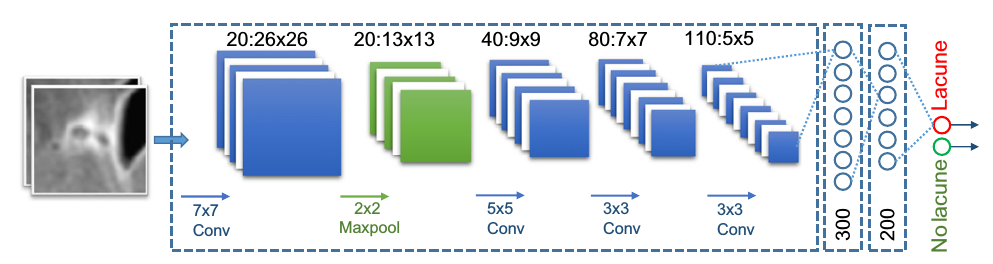
\includegraphics[width=\linewidth]{../Thesis_Docs/Images/5_ghafoorian_model1.png}
\end{figure}
\item Three adjustments:
\begin{itemize}
\item Extract soft tissue from T1-weighted scans.
\item Increase proportion of negative samples from 67\% to 91\%.
\item Remove downsampling from the first convolutional layer.
\end{itemize}
\end{itemize}
\end{frame}




% Our model adapts this existing model to the data set available from the Neuroscience department. The data set contains 411 MRI scans, of which 35 of these contain at least one lacune. Each image has two weightings - T1 and FLAIR. The coordinates of lacunes were determined by manually searching the T1 and FLAIR images for lesions that matched those described in an accompanying spreadsheet.
% One major difference our model makes is the form of the input data. Ghafoorian's model takes in T1-weighted and FLAIR inputs, applying some pre-processing to remove identifiers such as skull and eyes. 
\begin{frame}{Model evaluation}
\begin{itemize}
    \begin{block}{Sensitivity and Specificity}
	\[
		Sensitivity = P(Correct | Positive)
	\]
	\[
		Specificity = P(Correct | Negative)
	\]
    \end{block}
\item The full model by Ghafoorian et al. exhibited a sensitivity of 97.4\% and averaged 0.13 false-positives per cross-sectional image.
\end{itemize}

\end{frame}



%Our data set undergoes similar de-identification, whilst also removing CSF. Since lacunes have a similar signal intensity to CSF, this means that a lot of region surrounding lacunes is removed from the T1-weighted scans. Added effect of enlarging and emphasising the loss in intensity. Note that the flair images are extracted by masking a rectangular region rather than removing CSF, and so the intensities around lacunes are still visible.
%\begin{frame}{Results of data preprocessing}
%\begin{figure}
%\centering
%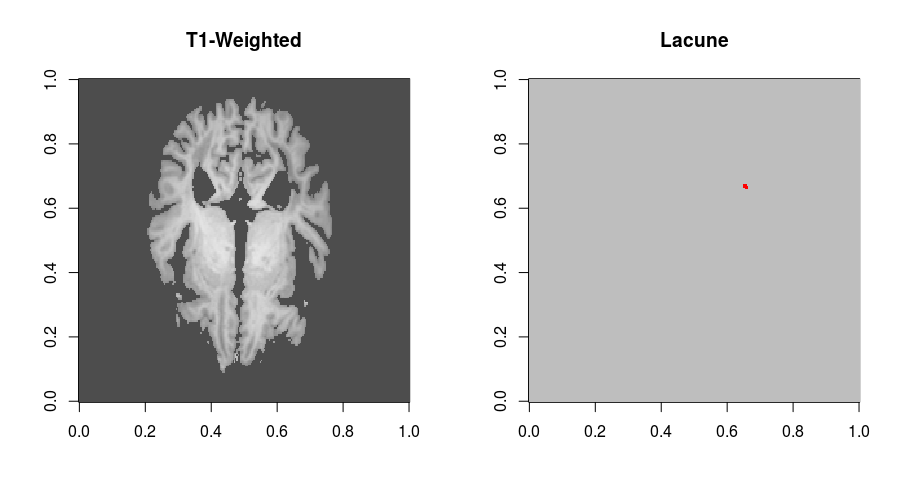
\includegraphics[width=\linewidth]{../Thesis_Docs/Images/6_soft_lacune.png}
%\end{figure}
%\end{frame}




% Samples were collected by extracting 51x51 T1-weighted and FLAIR images. As there are relatively few positive lacune samples, all possible samples were taken. Negatives were collected by sampling randomly within the brain region. Total of just over 40,000 samples. Positive samples make up 9\% of the data set. These samples were split into three: training, validation and testing sets. The model by Ghafoorian samples enough negatives such that positives make one-third of the data set. A model that tests this positive-negative ratio is discussed further in my thesis.
\begin{frame}{Sampling}
\begin{itemize}
\item Samples of 51$\times$51 resolution T1-weighted and \textsc{flair} images.
\item Positive samples were generated from all available lacunes.
\item Negative samples chosen randomly through the brain matter.
\item Total of over 40,000 samples split into training, validation and testing data sets.
\end{itemize}
\begin{figure}
\centering
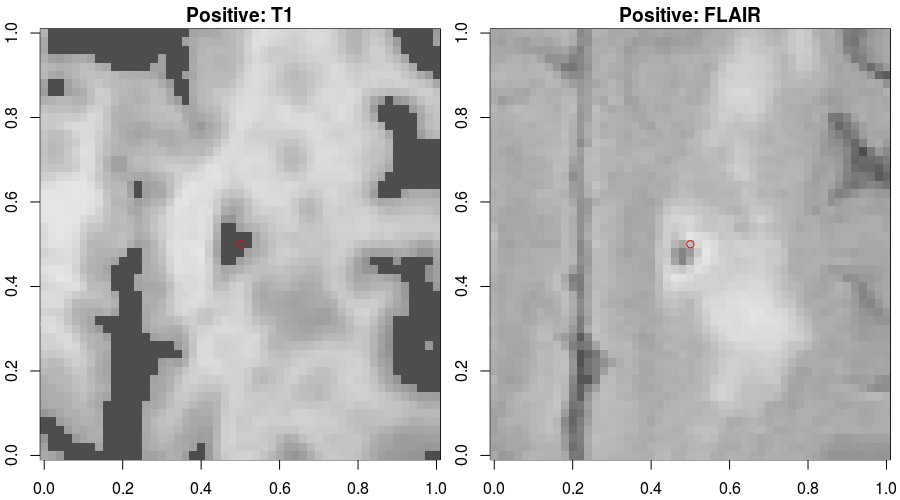
\includegraphics[scale=0.37]{../Thesis_Docs/Images/6_positive.png}
\end{figure}
\end{frame}


\section{Results}


% Now we apply our data to just the candidate detection component of the model. As is typical during neural network training, the training accuracy of the model exhibits overfitting and reaches 100\% in the first few epochs. What is more important here is the validation accuracy. 
\begin{frame}{Model training}
\begin{itemize}
\item Model overfits the training data quickly.
\end{itemize}
\begin{figure}
\centering
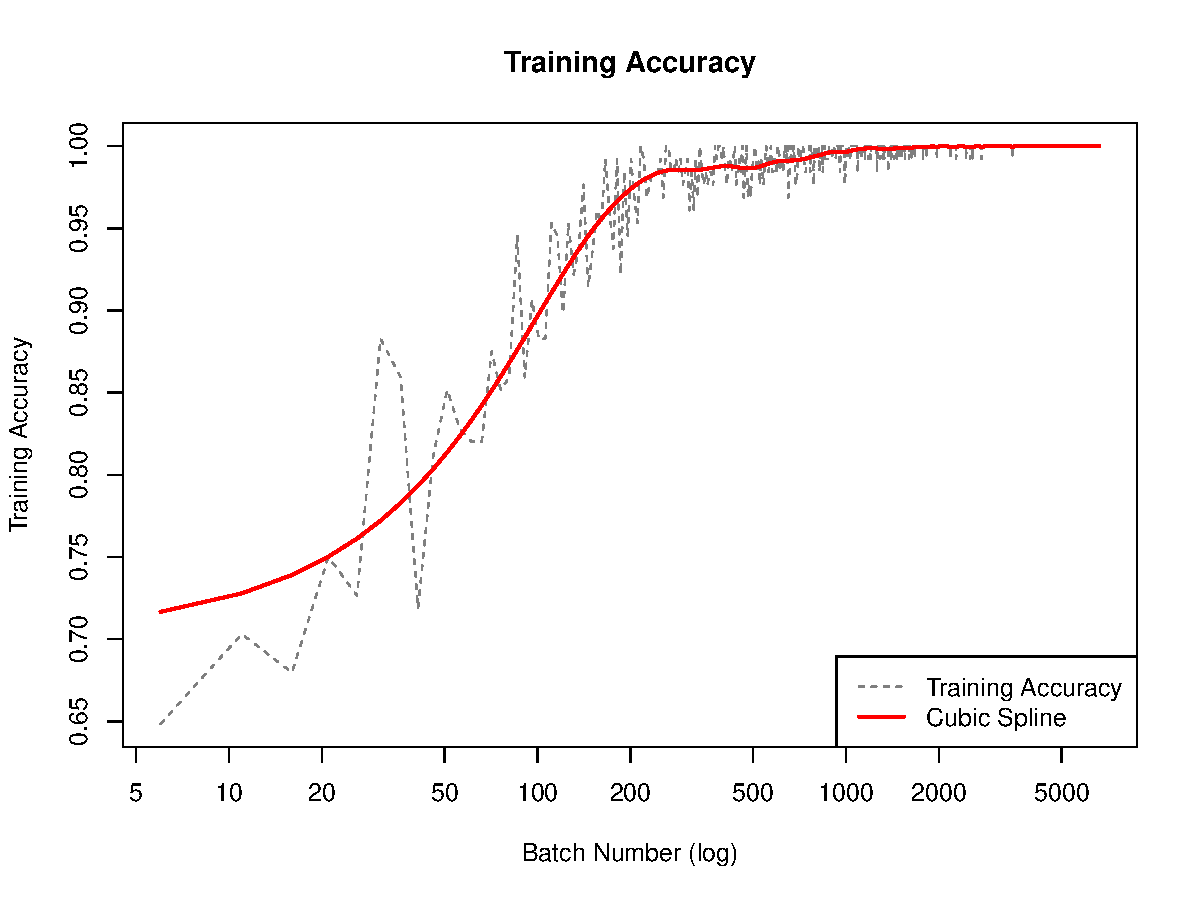
\includegraphics[width=0.83\linewidth]{../Thesis_Docs/Images/7_train_acc5.pdf}
\end{figure}
\end{frame}




% At each epoch, the model was tested against a separate data set, to assess how the model performs given data that wasn't use during training. This is the model's ability to detect something new. The model reaches its highest validation accuracy within 30 epochs. The model was saved at this point, despite attaining the same accuracy later on, to reduce any overfitting that may occur in later epochs. Generally as training epochs progress, we see validation accuracy begin to fall as the model really overfits the training data.
\begin{frame}{Model validation}
\begin{itemize}
\item Validation accuracy increases quickly.
\item The model was saved at the point of highest validation accuracy.
\end{itemize}
\begin{figure}
\centering
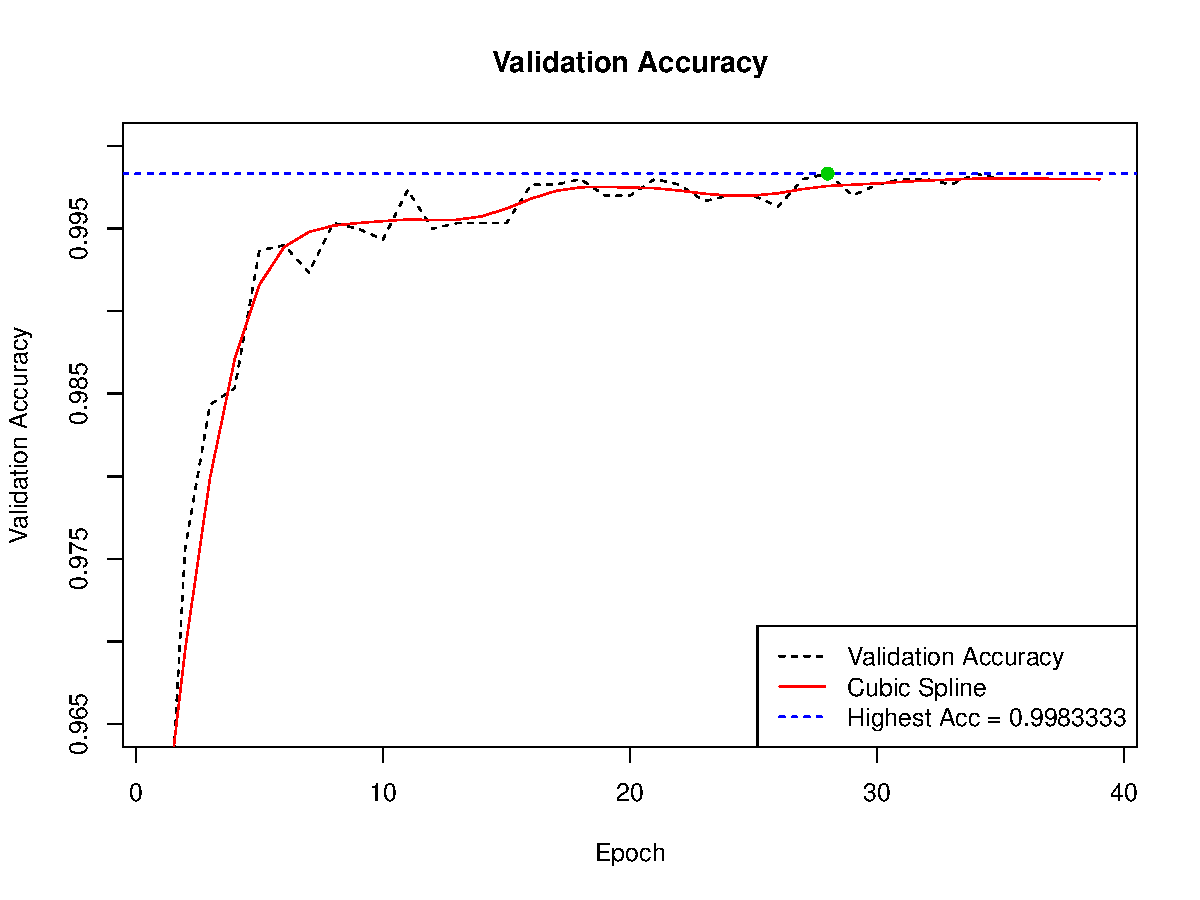
\includegraphics[width=0.83\linewidth]{../Thesis_Docs/Images/7_valid_acc5.pdf}
\end{figure}
\end{frame}





% Finally, this model was tested against the testing data set. Tabulating the true and false positives and negatives, we retrieve this confusion matrix. The key error we want to minimise here is the rate of false-negatives. These are lacunes that have been missed. Though undesirable, false-positives can be inspected and classified by a clinician within a reasonable amount of time, so long as there aren't too many of them. The final model exhibits a sensitivity of 99.9\% and specificity of 99.8\%. There are two main reactions from these figures. The first is that of success, the model is doing very well. The second is that of skepticism. Generally after building a model, accuracies at 100\% generally implies that something has gone wrong during the sampling process. For instance, the response has accidentally been fed into the model as a variable, or some issues with the methods of sampling. I have checked for this possibility in my code, and the data set, once generated, was randomised. The model does not have access to the surrounding classifications.
\begin{frame}{Results}
\begin{itemize}
\item Finally, the model is applied to the testing data set.
\end{itemize}
\begin{table}[ht]
	\centering
	\begin{tabular}{@{}lll@{}}
	\toprule[1.5pt]
	& Positive & Negative\\
	\midrule
	True & 961 & 9977\\
	False & 19 & 1\\
	\bottomrule[1.5pt]\\
	\end{tabular}
\end{table}
\begin{itemize}
\item Gives testing sensitivity of 99.9\% and specificity of 99.8\%.
\pause
\item Are these results too good?
\end{itemize}
\end{frame}




% To alleviate some concerns, we now take a look at some examples of correctly and incorrectly classified points. Examples of true positives. Regions of zero or low intensity in T1, whilst having a dark region surrounded by hyperintensity in flair. If we take a look at some false-positives, we see that they exhibit this same structure. Low to zero T1, near a dark region with hyperintense edge in flair. False-negatives are rare. In this instance, the lacune is very small, only 3 mm in diameter. So small that there is no hyperintense rim visible in the flair image.
\begin{frame}{Examination of true-positives}
\begin{itemize}
\item Model appears to be detecting dark regions in T1 and bright edges in \textsc{flair}.
\end{itemize}
\begin{figure}
\centering
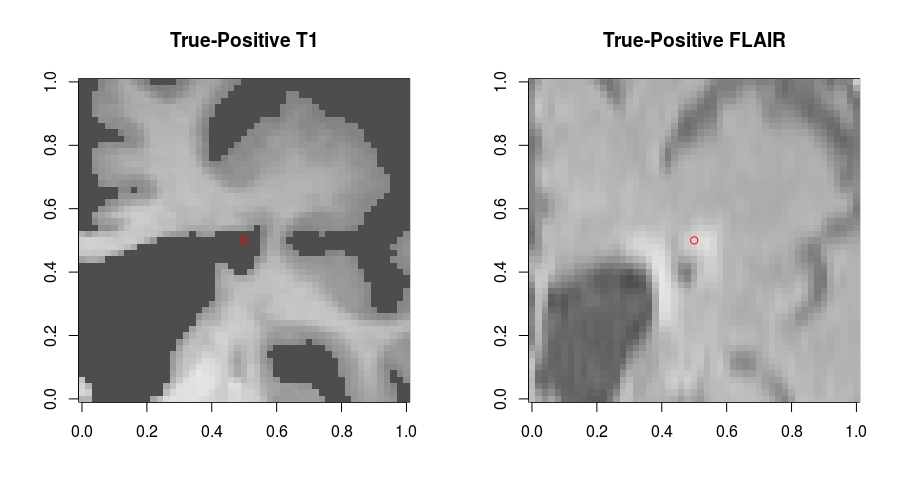
\includegraphics[width=\linewidth]{../Thesis_Docs/Images/7_TP_t1_flair.png}
\end{figure}
\end{frame}

\begin{frame}{Examination of false-positives}
\begin{itemize}
\item Model appears to be detecting dark regions in T1 and bright edges in \textsc{flair}.
\end{itemize}
\begin{figure}
\centering
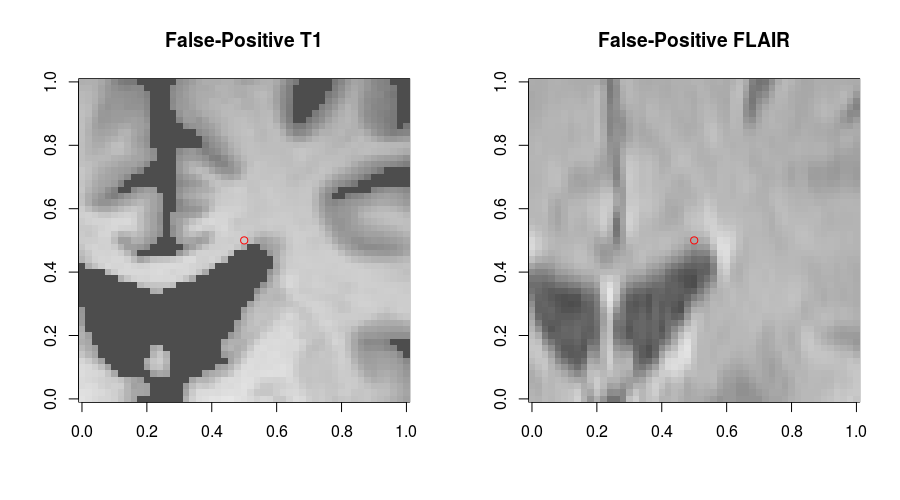
\includegraphics[width=\linewidth]{../Thesis_Docs/Images/7_FP_t1_flair2.png}
\end{figure}
\end{frame}

\begin{frame}{Examination of false-negatives}
\begin{itemize}
\item Model misclassifies a small lacune with no bright edges in \textsc{flair}.
\end{itemize}
\begin{figure}
\centering
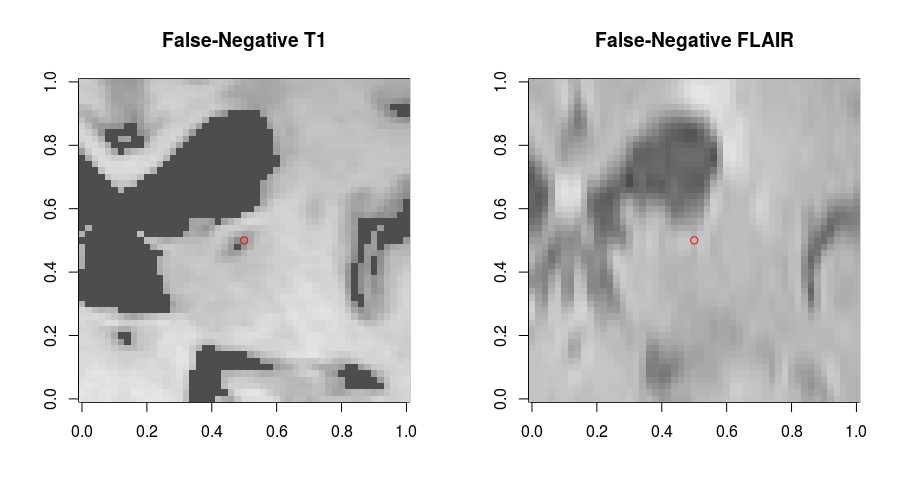
\includegraphics[width=\linewidth]{../Thesis_Docs/Images/7_FN_t1_flair.png}
\end{figure}
\end{frame}


% Conclusion. Successfully developed a machine learning algorithm that can identify lacunes from soft tissue extracted T1-weighted images and corresponding flair. Further research: Though 99.8\% specificity is high, there are a large number of voxels in a brain scan, so there may still be a considerable number of false-positives. Worth feeding model through the three-dimensional cnn. Note the extra computation and data collection time required. Also worth experimenting with the threshold during soft tissue extraction. The edges of the mask were quite harsh and lost a lot of data beyond just the eyes and skull. Setting it so that it retains more CSF also retain more of the brain matter which could help reduce false positives. CNNs are computationally and storage intensive. Millions of variables. Worth exploring other types of models, such as gradient boosting through XGBoost. 
\begin{frame}{Conclusion and future research}
\begin{itemize}
\item Model successfully identifies lacunes with a very high accuracy, efficiency and consistency.
\item Improves validity of inference concerning strokes originating from lacunes.
\item Further research could reduce false-positives by:
\begin{itemize}
\item Applying a three-dimensional \textsc{cnn}.
\item Assessing the benefit of location-based variables.
\end{itemize}
\end{itemize}

\end{frame}


\begin{frame}[allowframebreaks]{References}
	\bibliographystyle{plainnat}
	\bibliography{bibliography_pres.bib}
\end{frame}




\end{document}


